\begin{figure*}[t]
    \centering
    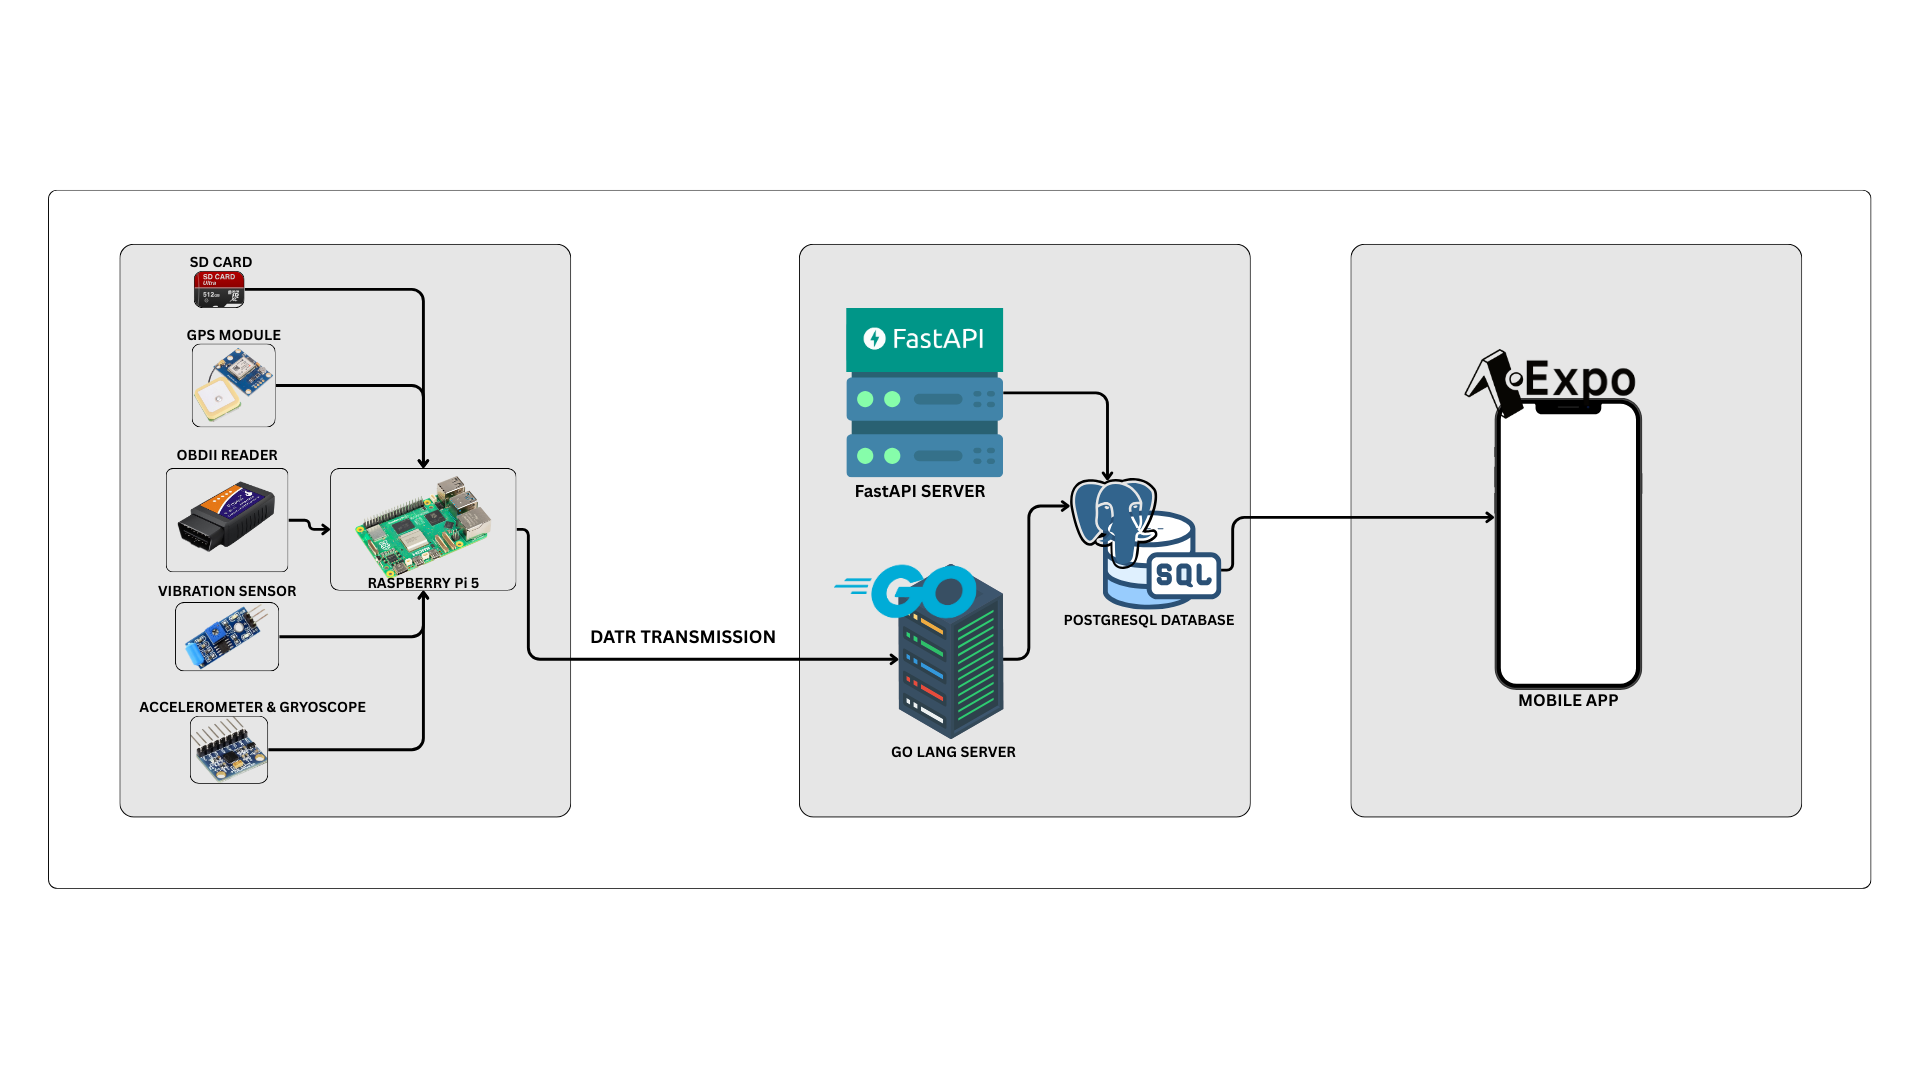
\includegraphics[width=\textwidth]{assets/System_design.png}
    \caption{System architecture of the proposed Automotive Diagnostic and Activity Monitoring (ADAM) system.}
    \label{fig:system_architecture}
\end{figure*}

\section{Methodology}
The proposed vehicle diagnostic and driver behaviour analysis system integrates various components of hardware and software to collect real time data collection for analysis and user analysis. The architecture is designed to collect vehicle information via obd II port, transmit it wirelessly to cloud server for processing and provides a visual representation of processed data through a mobile application.

The system consists of 4 primary components:
obd-II data collection and transmission
data analysis using machine learning models
cross platform mobile application
A block diagram representing the overall system architecture and data flow from vehicle sensors to end user presentation is shown in figure 1.1


We have utilize an obd-II interface device compatible with standard protocols such as CAN( ISO 15765-4) and K-Line (ISO 9141-2). The device communicates with a raspberry pi 5 (a single-board computer),which is used for data collection along with other sensors like neo 6m gps module, sw 420 vibration sensor, mpu 6050 gyroscope/acceleration module. the data which is collected is stored in micro sd which can be used for forensic analysis.

we have implemented four machine learning models that predict based on data are:
 driver behaviour analysis,fuel consumption, predictive maintenance,engine health performance

    
      